\chapter[Results]{Results}
\label{cp:results}

{
	\parindent0pt
	The data collected as part of the evaluation of this work is presented and discussed in this section. The hardware and software setup used are given in \autoref{sec:experimental_setup}, as to allow for reproducibility of our results. Sections \ref{sec:experimental_setup} and \ref{sec:justification_rebuild} discuss some implementation choices based on collected data. Finally, the benchmark results for each scenario are presented in \autoref{sec:benchmarking_results}.
}

% TODO: How do results differ based on tuning strategy? Full-search vs. others
\section{Experimental Setup}
\label{sec:experimental_setup}
The measurements collected for analysis in this chapter were obtained on the CoolMUC4 Linux-Cluster of the Leibniz\-/Rechenzentrum\footnote{\href{https://www.lrz.de/}{https://www.lrz.de/}}. The nodes in the \texttt{cm4} cluster consist of processors in the Sapphire Rapids family (Intel\textsuperscript{\textregistered} Xeon\textsuperscript{\textregistered} Platinum 8480+)  with \qty{2.1}{\gibi \byte} of memory per logical CPU and \qty{488}{\gibi \byte} per node \cite{LSC2025}. For benchmarking purposes, the AutoPas library and \texttt{md-flexible} were compiled with  Spack GCC 13.2.0 and Intel MPI 2021.12.0 on commit \texttt{46bb925c8c5827faee8691afefd9f714630f20f1}.

The scripts used to generate the Slurm jobs and configuration files can be found in the repository of this thesis\footnote{\href{https://github.com/ladnik/bachelor-thesis}{https://github.com/ladnik/bachelor-thesis}}.

% TODO: add version compiler/mpi version, add commit hash

% Refer to Appendix for additional data
% Refer to Input files
\section{Choice of Simulation Statistics}
\label{sec:justification_rebuild}
As referred to before in \autoref{sec:avail_sim_stats}, there are several simulation statistics available upon which trigger strategies could be based. Even the iteration runtimes themselves are differentiated into multiple parameters: the time spent on computing interactions, traversing remainders and rebuilding neighbor lists.

In this thesis, we will consider the sum of these times with the exception of the rebuilding measurements. This choice can be justified by inspecting runtime data we collected: As shown  in \autoref{fig:rebuild_times}, the rebuild times remain constant over all iterations simulated with a particular configuration. Their inclusion therefore does not provide any new information, but rather smooths out the overall measurements and thus decreases the effectivity at which a scenario change can be detected.

Additionally, in scenarios with a low average number of neighbors, the rebuilding of neighbor lists takes longer than the interaction computations. Considering that the rebuilding only happens in iterations that are a multiple of \texttt{rebuildFrequency}, this leads to stability problems in trigger strategies with a low number of samples, as the few rebuild iterations greatly outweigh all non-rebuild iterations.

\begin{figure}[htpb]
	\begin{subfigure}{0.5\textwidth}
		\centering
		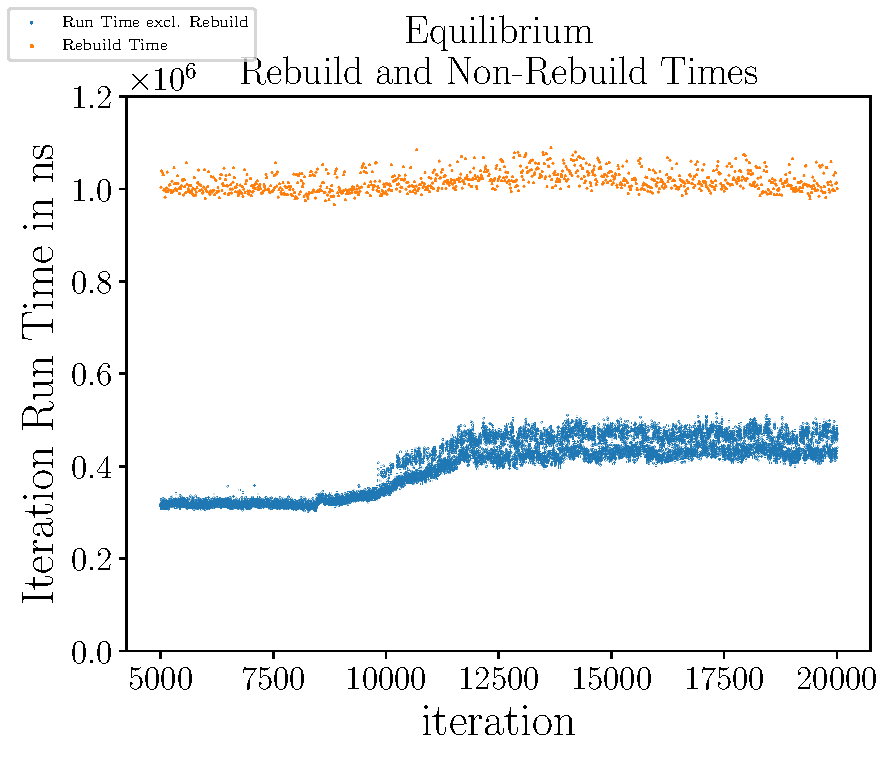
\includegraphics[width=\textwidth]{./Figures/plots/equilibrium_rebuild.pdf}
	\end{subfigure}
	\begin{subfigure}{0.5\textwidth}
		\centering
		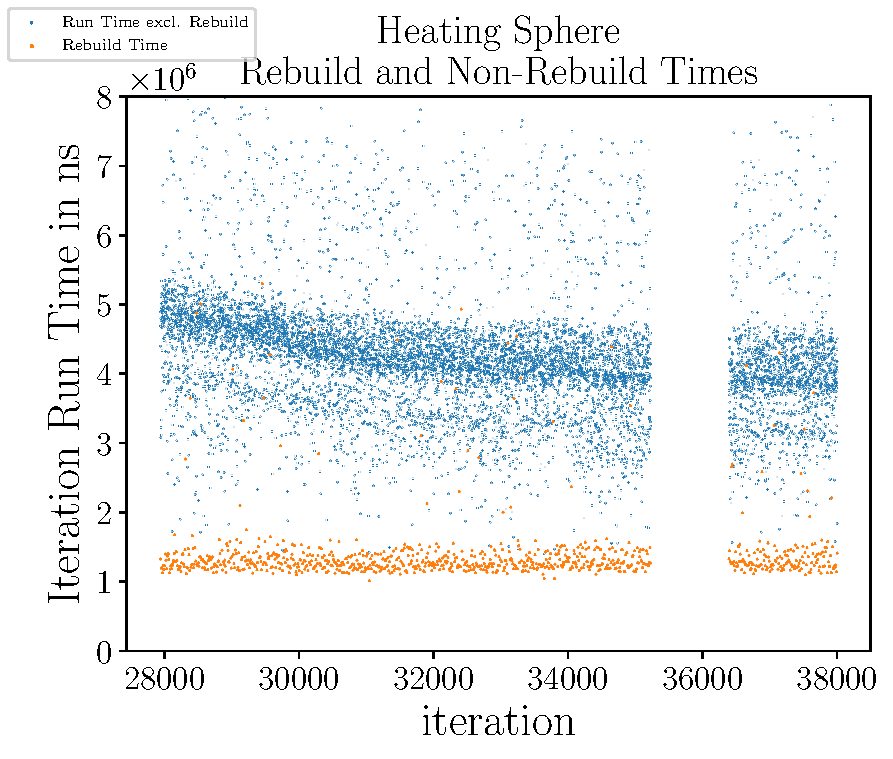
\includegraphics[width=\textwidth]{./Figures/plots/hs_rebuild.pdf}
	\end{subfigure}
	\caption{Rebuild and non-rebuild times in the equilibrium (left) and heating-sphere (right) scenario. [TODO]}
	\label{fig:rebuild_times}
\end{figure}



\section{Computational Overhead}
\label{sec:overhead_results}
Our strategies analyze data at runtime and therefore \textellipsis

To quantify the overhead our strategies introduce, we compare runs with a single initial tuning phase. That way, we remove any changes in runtime that may occur due to different tuning phase initiation points of our strategies. To achieve this, we use a factor high enough, such that none of our strategies initiate a new tuning phase. For the baseline run, we use static tuning intervals with a \texttt{tuning-interval} set longer than the total number of iterations to simulate, which results in a single tuning phase starting in iteration \num{0}. \autoref{fig:overhead_comparison} shows the overhead obtained that way for the equilibrium scenario with $\lambda=50$ and $n=500$.


% TODO: integrate this
To exemplify the importance of optimizing the trigger routines, \autoref{fig:optimization_speedup} illustrates the runtime differences between naive and optimized triggers in the equilibrium scenario. The naive version recalculates the average over all samples each iteration, whereas the optimized version uses a ring buffer and running summation to reduce computational cost.
The speedup experienced is not only due to a lowering of computational overhead, but also due to less tuning iterations. This fact can be explained by the aforementioned self influence of the triggers: higher overhead might lead to higher fluctuation in iteration runtime which in turn leads to unstable trigger behavior, especially in the averaging trigger.

% TODO: check if this makes any sense

\begin{figure}[htpb]
	\tikzset{
		barstyle1/.style={fill=tumblueaccmedium, draw=chaptertumblue},
		barstyle2/.style={pattern color=tumblueaccmedium, draw=chaptertumblue, pattern=north east lines},
	}
	\begin{subfigure}{0.5\textwidth}
		\centering
		\begin{tikzpicture}
			\def\barwidth{15pt}
			\begin{axis}[
					height=0.8\textwidth,
					width=\textwidth,
					xlabel={Trigger Strategy},
					ylabel={Overhead in \%},
					enlarge x limits=0.1,
					ymin=0,
					symbolic x coords={Simple,Avg,Split,Regression},
					xtick=data,
					bar width=\barwidth,
					legend entries={Overhead}
				]

				\addlegendimage{legend image code/.code={
							\draw[barstyle1, anchor=center] (0cm, -0.15cm)  rectangle (0.3cm,0.15cm);
						}}
				\addlegendentry{\scriptsize Overhead}

				% overheads
				\addplot[ybar, barstyle1] coordinates {
						(Simple,0)
						(Avg,0)
						(Split,0)
						(Regression,0)
					};
			\end{axis}
		\end{tikzpicture}
		\subcaption{Overhead of the various trigger strategies. [TODO]}
		\label{fig:overhead_comparison}
	\end{subfigure}%
	\begin{subfigure}{0.5\textwidth}
	\centering
	\begin{tikzpicture}
		\def\barwidth{15pt}
		\begin{axis}[
			height=0.8\textwidth,
			width=\textwidth,
			xlabel={Trigger Strategy},
			ylabel={Total Runtime in \unit{ns}},
			enlarge x limits=0.25,
			symbolic x coords={Avg,Split,Regression},
			xtick=data,
			bar width=\barwidth,
			legend entries={Unoptimized, Optimized}
			]
			
			\addlegendimage{legend image code/.code={
					\draw[barstyle1, anchor=center] (0cm, -0.15cm)  rectangle (0.3cm,0.15cm);
			}}
			\addlegendentry{\scriptsize Unoptimized}
			\addlegendimage{legend image code/.code={
					\draw[barstyle2, anchor=center] (0cm, -0.15cm)  rectangle (0.3cm,0.15cm);
			}}
			\addlegendentry{\scriptsize Optimized}
			
			% unoptimized average
			\addplot[ybar, bar shift=-0.5*\barwidth, barstyle1] coordinates {
				(Avg,1694063817546)
				(Split,1141728867654)
				(Regression,1112338563086)
			};
			% optimized average
			\addplot[ybar, bar shift=0.5*\barwidth, barstyle2] coordinates {
				(Avg,962648240758)
				(Split,999681150940)
				(Regression,889891999680)
			};
		\end{axis}
	\end{tikzpicture}
	\subcaption{Average Speedup between unoptimized and optimized runs.}
	\label{fig:optimization_speedup}
\end{subfigure}
	\caption{TODO}
\end{figure}
%TODO: add speedup after optimization (self influence of runtime)


\tikzset{
	linestyleA/.style={chaptertumblue, densely dotted, thick},
	linestyleB/.style={tumblueaccdark, densely dashed, thick},
	linestyleC/.style={tumblueaccmedium, solid, thick},
	linestyleD/.style={tumblueacclight, densely dashdotted, thick},
}

\pgfplotsset{
	triggerplot/.style={
			height=0.7\textwidth,
			width=\textwidth,
			xlabel={Trigger Factor $\lambda$},
			xtick={1.25, 1.5, 1.75},
			legend style={font=\small},
			legend cell align=center,
			legend columns=3,
			legend style={at={(0.5,1.03)}, anchor=south, fill=none, draw=none, align=center},
			legend image post style={xscale=0.5},
			ylabel near ticks},
	logtriggerplot/.style={
			triggerplot,
			log basis y = 10,
			log ticks with fixed point}
}




\section{Benchmarking Results}
\label{sec:benchmarking_results}
% Formula for deviation from static baseline:
% ROUND((stat_val/dyn_val - 1)*100)

The speedups presented in the following plots was computed by the formula given in \eqref{eq:speedup_formula}, where $t_\text{baseline}$ represents the runtime with tuning phases at fixed intervals and $t_\text{dynamic}$ the runtime of our implementation.
\begin{equation}
	\text{S}=\frac{t_\text{baseline}}{t_\text{dynamic}}-1\label{eq:speedup_formula}
\end{equation}

% TODO: where to place this
The blue bars in the graphs represent the runtime of that particular iteration.
In the configuration plots, the colored background identifies the used configuration: same configurations map to the same color. The gaps in the plot are where tuning iterations have been logged -- as their runtime is not relevant for the scenario change and would distort the actual runtime plot, they are not reported here. The red vertical lines indicate the start of a tuning phase.

\subsection{Equilibrium}
\subsubsection{Speedup and Default Parameters}

As can be seen in \autoref{fig:params_equil}, a trigger factor of $\lambda=1.5$ leads to increased speedup compared to $\lambda=1.25$ in nearly all triggering strategies. This is however mainly due to the nature of the equilibrium scenario: after the initial configuration selection, the optimal configuration is not expected to change.
Therefore, not initiating any new tuning phases will lead to a decrease in total simulation runtime. That the speedup is indeed  a result of the decreased number of tuning iterations can be verified by looking at the right-hand side plots; for the simple and averaging trigger it is most noticeable.
Additionally, triggers with a larger sample size will typically trigger less frequently, as more of the variability in iteration runtime is smoothed out. For a too large number of samples, the speedup decreases however, as the computational overhead is directly proportional to the number of samples.
% TODO: rewrite
%This is best seen in the plots for the regression trigger, as the share of tuning iterations remains constant for all sample sizes, but the speedup decreases. Especially for the regression triggers, the computations required per sample and in each iteration are significant.

%The increase of th enumber of tuning iterations as seen in the split trigger with $n=250$ can be explained by \textellipsis
% TODO: self-interaction
% TODO: longer intervals -> slower reaction?

\begin{figure}[htpb]
	\centering
	\begin{subfigure}{0.45\textwidth}
		\begin{tikzpicture}
			\begin{axis}[
					triggerplot,
					legend columns=2,
					ylabel={Speedup \%},
				]
				% TimeBasedSimple
				\addplot[linestyleD] coordinates{
						(1.25,-5)
						(1.5,12)
						(1.75,5)};
				% TimeBasedAverage 1000
				\addplot[linestyleA] coordinates{
						(1.25,21)
						(1.5,44)
						(1.75,47)};
				% TimeBasedAverage 500
				\addplot[linestyleB] coordinates{
						(1.25,10)
						(1.5,34)
						(1.75,47)};
				% TimeBasedAverage 250
				\addplot[linestyleC] coordinates{
						(1.25,17)
						(1.5,26)
						(1.75,34)};
				\legend{Simple,Avg-1000,Avg-500,Avg-250}
			\end{axis}
		\end{tikzpicture}
		%		\subcaption{Simple and Average Triggers}
	\end{subfigure}
	\hspace{0.05\textwidth}
	\begin{subfigure}{0.45\textwidth}
		\begin{tikzpicture}
			\begin{axis}[
					logtriggerplot,
					legend columns=2,
					ylabel={Tuning Iterations \%},
					ymode=log,
					ymin=1,
					ymax=100,
				]
				% TimeBasedSimple
				\addplot[tumblueacclight, thick] coordinates{
						(1.25,29.37)
						(1.5,2.26)
						(1.75,2.26)};
				% TimeBasedAverage 1000
				\addplot[linestyleA] coordinates{
						(1.25,2.26)
						(1.5,1.51)
						(1.75,1.51)};
				% TimeBasedAverage 500
				\addplot[linestyleB] coordinates{
						(1.25,2.26)
						(1.5,2.26)
						(1.75,1.51)};
				% TimeBasedAverage 250
				\addplot[linestyleC] coordinates{
						(1.25,2.26)
						(1.5,1.51)
						(1.75,1.51)};
				\legend{Simple,Avg-1000,Avg-500,Avg-250}
			\end{axis}
		\end{tikzpicture}
		%		\subcaption{Simple and Average Triggers}
	\end{subfigure}
	\begin{subfigure}{0.45\textwidth}
		\begin{tikzpicture}
			\begin{axis}[
					triggerplot,
					ylabel={Speedup \%},
				]
				% TimeBasedSplit 1000
				\addplot[linestyleA] coordinates{
						(1.25,42)
						(1.5,46)
						(1.75,35)};
				% TimeBasedSplit 500
				\addplot[linestyleB] coordinates{
						(1.25,43)
						(1.5,38)
						(1.75,40)};
				% TimeBasedSplit 250
				\addplot[linestyleC] coordinates{
						(1.25,-6)
						(1.5,28)
						(1.75,-7)};
				\legend{Split-1000,Split-500,Split-250}
			\end{axis}
		\end{tikzpicture}
		%		\subcaption{Split Trigger}
	\end{subfigure}
	\hspace{0.05\textwidth}
	\begin{subfigure}{0.45\textwidth}
		\begin{tikzpicture}
			\begin{axis}[
					logtriggerplot,
					ylabel={Tuning Iterations \%},
					ymode=log,
					ymin=1,
					ymax=100,
				]
				% TimeBasedSplit 1000
				\addplot[linestyleA] coordinates{
						(1.25,3.77)
						(1.5,3.01)
						(1.75,3.77)};
				% TimeBasedSplit 500
				\addplot[linestyleB] coordinates{
						(1.25,4.52)
						(1.5,4.52)
						(1.75,3.77)};
				% TimeBasedSplit 250
				\addplot[linestyleC] coordinates{
						(1.25,81.7)
						(1.5,6.03)
						(1.75,81.9)};
				\legend{Split-1000,Split-500,Split-250}
			\end{axis}
		\end{tikzpicture}
		%		\subcaption{Split Trigger}
	\end{subfigure}
	\begin{subfigure}{0.45\textwidth}
		\begin{tikzpicture}
			\begin{axis}[
					triggerplot,
					legend columns=2,
					ylabel={Speedup \%},
				]
				% TimeBasedRegression 2000
				\addplot[linestyleA] coordinates{
						(1.25,-3)
						(1.5,13)
						(1.75,14)};

				% TimeBasedRegression 1500
				\addplot[linestyleB] coordinates{
						(1.25,-4)
						(1.5,14)
						(1.75,15)};

				% TimeBasedRegression 1000
				\addplot[linestyleC] coordinates{
						(1.25,7)
						(1.5,15)
						(1.75,14)};

				% TimeBasedRegression 500		
				\addplot[linestyleD] coordinates{
						(1.25,5)
						(1.5,16)
						(1.75,15)};

				\legend{Reg-2000,Reg-1500,Reg-1000,Reg-500}
			\end{axis}
		\end{tikzpicture}
		%		\subcaption{Regression Trigger}
	\end{subfigure}%
	\hspace{0.05\textwidth}
	\begin{subfigure}{0.45\textwidth}
		\begin{tikzpicture}
			\begin{axis}[
					logtriggerplot,
					legend columns=2,
					ylabel={Tuning Iterations \%},
					ymode=log,
					ymin=1,
					ymax=100,
				]
				% TimeBasedRegression 2000
				\addplot[linestyleA] coordinates{
						(1.25,18.72)
						(1.5,4.32)
						(1.75,1.44)};

				% TimeBasedRegression 1500
				\addplot[linestyleB] coordinates{
						(1.25,19.37)
						(1.5,1.44)
						(1.75,1.44)};

				% TimeBasedRegression 1000
				\addplot[linestyleC] coordinates{
						(1.25,7.88)
						(1.5,1.44)
						(1.75,1.44)};

				% TimeBasedRegression 500		
				\addplot[linestyleD] coordinates{
						(1.25,10.08)
						(1.5,1.44)
						(1.75,1.44)};

				\legend{Reg-2000,Reg-1500,Reg-1000,Reg-500}
			\end{axis}
		\end{tikzpicture}
		%		\subcaption{Regression Trigger}
	\end{subfigure}%
	\caption{Trigger behavior in the equilibrium scenario, the numbers in the legends refer to the number of samples $n$ considered. Note the logarithmic scale in the plots on the right hand side.}
	\label{fig:params_equil}
\end{figure}

The collected data suggests default parameters as presented in \autoref{tab:equil_defaults}.
\begin{table}[htpb]
	\centering
	\begin{tabular}{lcc}
		\toprule
		\textbf{Trigger}             & \textbf{Trigger factor $\lambda$} & \textbf{Number of samples $n$} \\ [0em]
		\midrule
		\texttt{TimeBasedSimple}     & $1.5$                             & --                             \\
		\texttt{TimeBasedAverage}    & $1.75$                            & 500                            \\
		\texttt{TimeBasedSplit}      & $1.5$                             & 1000                           \\
		\texttt{TimeBasedRegression} & $1.5$                             & 500                            \\
		\bottomrule
	\end{tabular}
	\caption{Suggested default parameters for the equilibrium scenario.}
	\label{tab:equil_defaults}
\end{table}


\subsubsection{Selected Runs}
% TODO: fix plots
\begin{figure}[htpb]
	\begin{subfigure}{0.5\textwidth}
		\centering
		% equilibrium_dynamic_TimeBasedRegression_1.25_1000
		%		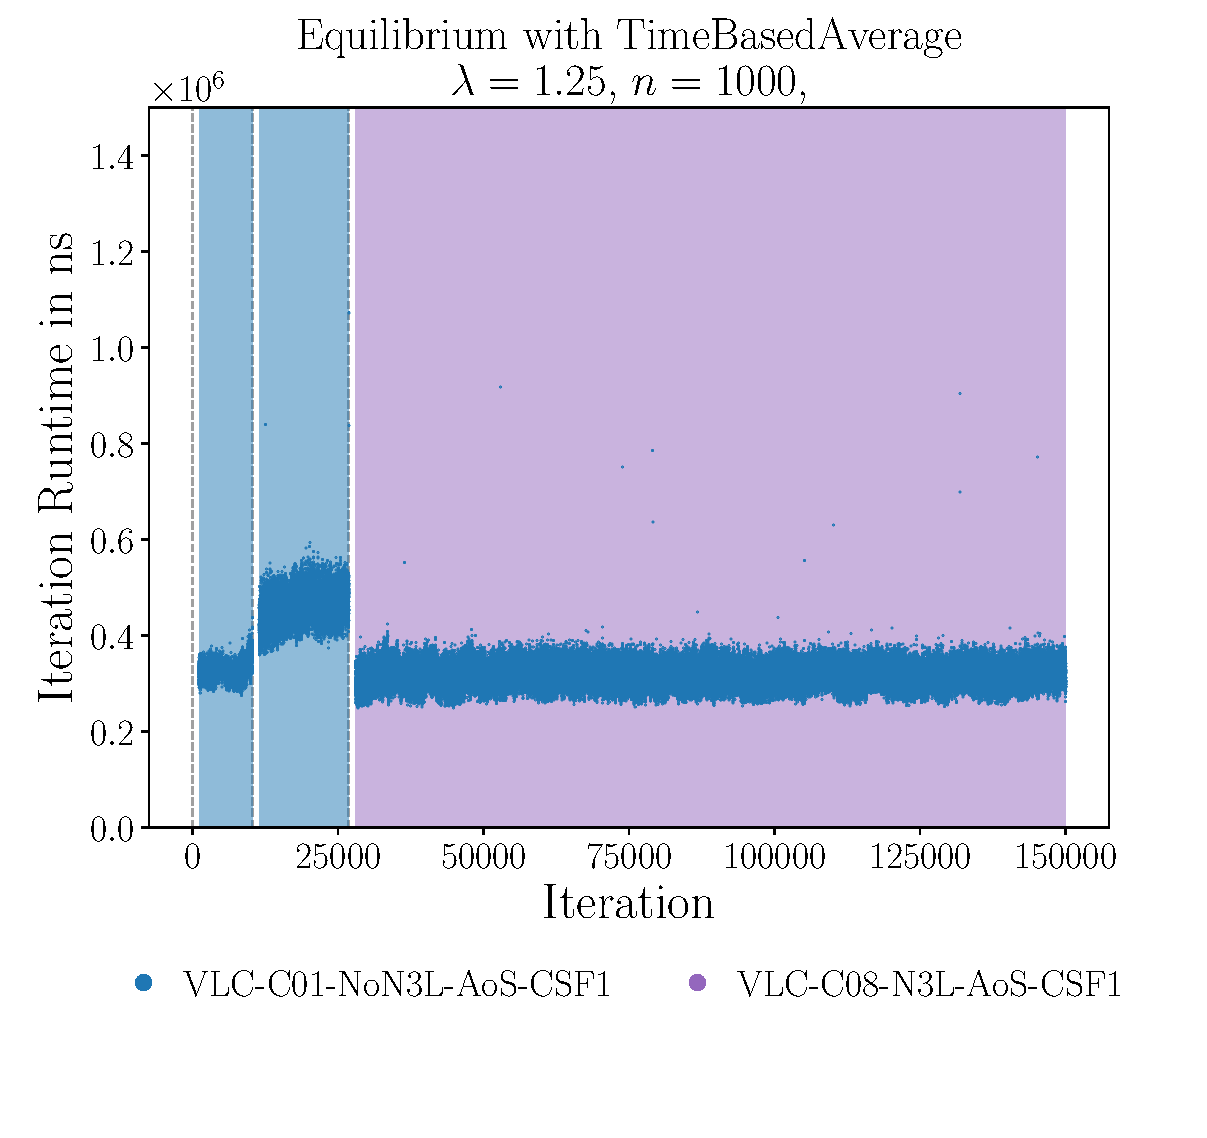
\includegraphics[width=\textwidth]{./Figures/plots/equilibrium_configs_good.pdf}
		\subcaption{Good scenario change detection with the regression-based trigger.}
	\end{subfigure}
	\begin{subfigure}{0.5\textwidth}
		\centering
		% TODO: heating sphere
		%		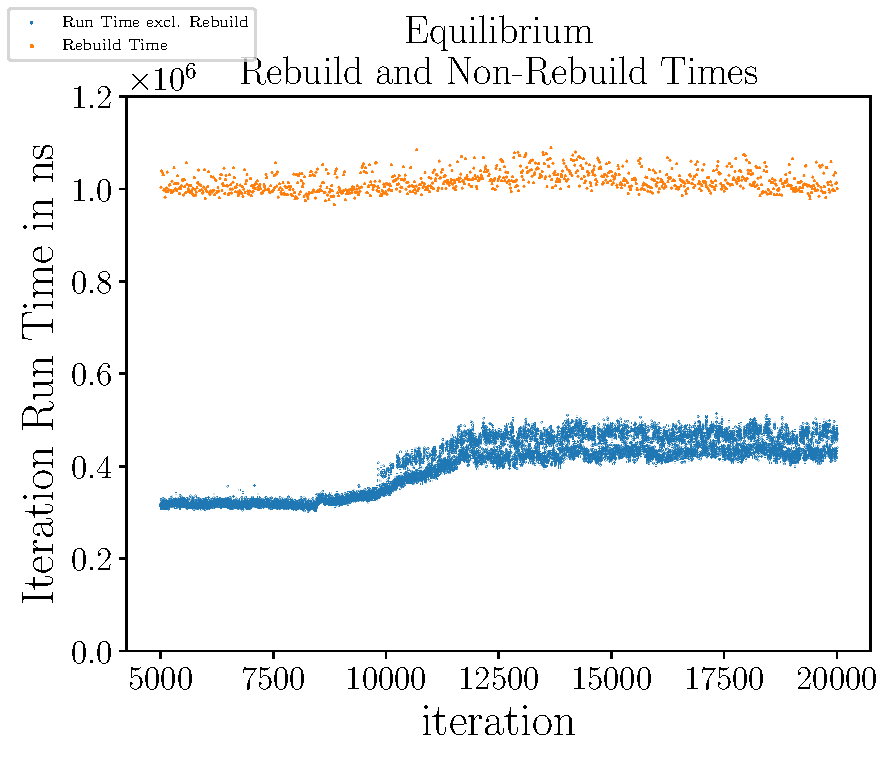
\includegraphics[width=\textwidth]{./Figures/plots/equilibrium_rebuild.pdf}
	\end{subfigure}
	\caption{Examples of trigger behavior in the equilibrium scenario.}
	\label{fig:equilibrium_trigger_behavior}
\end{figure}

\autoref{fig:equilibrium_trigger_behavior} shows two of the experimental runs in detail. On the left hand side, a \texttt{TimeBasedRegressionTrigger} with $\lambda=1.25$, $n=1000$ detects scenario change reliably. The first dynamically triggered tuning phase appears in iteration \num{9798}, which is due to the sharp increase in iteration runtime. Afterwards, the iteration runtimes do not increase fast enough to warrant any new trigger phase. The next tuning phase is therefore only triggered because of outliers around iteration \num{80000}, particularly iteration \num{86097} immediately before the trigger fires. Interestingly, even tough the scenario change wasn't detectible in the runtime itself, the next chosen configuration (\texttt{VLC-C01-NoN3L-AoS-CSF0.5}) performs better. The remaining tuning phases are again triggered by outliers.
% TODO: first maybe due to outliers too?


On the right hand side\textellipsis


Additional plots showing the behavior of various trigger strategies are included in the appendix.
% TODO: add plots to appendix, add ref


% TODO: mention Theil-Sein estimator


\subsubsection{Optimality}


\subsection{Exploding Liquid}
\subsubsection{Speedup and Default Parameters}

\subsubsection{Selected Runs}
\subsubsection{Optimality}

\subsection{Heating Sphere}
\subsubsection{Speedup and Default Parameters}

% TODO: check static run?

% TODO: Note that percentage of tuning iterations is higher, as simulation is shorter...

\begin{figure}[htpb]
	\centering
	\begin{subfigure}{0.45\textwidth}
		\begin{tikzpicture}
			\begin{axis}[
					triggerplot,
					legend columns=2,
					ylabel={Speedup \%},
				]
				% TimeBasedSimple
				\addplot[linestyleD] coordinates{
						(1.25,-17)
						(1.5,-16)
						(1.75,-11)};
				% TimeBasedAverage 1000
				\addplot[linestyleA] coordinates{
						(1.25,23)
						(1.5,28)
						(1.75,30)};
				% TimeBasedAverage 500
				\addplot[linestyleB] coordinates{
						(1.25,23)
						(1.5,23)
						(1.75,29)};
				% TimeBasedAverage 250
				\addplot[linestyleC] coordinates{
						(1.25,17)
						(1.5,19)
						(1.75,24)};
				\legend{Simple,Avg-1000,Avg-500,Avg-250}
			\end{axis}
		\end{tikzpicture}
		%		\subcaption{Simple and Average Triggers}
	\end{subfigure}
	\hspace{0.05\textwidth}
	\begin{subfigure}{0.45\textwidth}
		\begin{tikzpicture}
			\begin{axis}[
					logtriggerplot,
					legend columns=2,
					ylabel={Tuning Iterations \%},
					ymode=log,
					ymin=1,
					ymax=100,
				]
				% TimeBasedSimple
				\addplot[tumblueacclight, thick] coordinates{
						(1.25,98)
						(1.5,2.94)
						(1.75,85)};
				% TimeBasedAverage 1000
				\addplot[linestyleA] coordinates{
						(1.25,23)
						(1.5,19)
						(1.75,17)};
				% TimeBasedAverage 500
				\addplot[linestyleB] coordinates{
						(1.25,23)
						(1.5,23)
						(1.75,17)};
				% TimeBasedAverage 250
				\addplot[linestyleC] coordinates{
						(1.25,29)
						(1.5,27)
						(1.75,21)};
				\legend{Simple,Avg-1000,Avg-500,Avg-250}
			\end{axis}
		\end{tikzpicture}
		%		\subcaption{Simple and Average Triggers}
	\end{subfigure}
	\begin{subfigure}{0.45\textwidth}
		\begin{tikzpicture}
			\begin{axis}[
					triggerplot,
					ylabel={Speedup \%},
				]
				% TimeBasedSplit 1000
				\addplot[linestyleA] coordinates{
						(1.25,76)
						(1.5,76)
						(1.75,67)};
				% TimeBasedSplit 500
				\addplot[linestyleB] coordinates{
						(1.25,72)
						(1.5,76)
						(1.75,72)};
				% TimeBasedSplit 250
				\addplot[linestyleC] coordinates{
						(1.25,68)
						(1.5,72)
						(1.75,76)};
				\legend{Split-1000,Split-500,Split-250}
			\end{axis}
		\end{tikzpicture}
		%		\subcaption{Split Trigger}
	\end{subfigure}
	\hspace{0.05\textwidth}
	\begin{subfigure}{0.45\textwidth}
		\begin{tikzpicture}
			\begin{axis}[
					logtriggerplot,
					ylabel={Tuning Iterations \%},
					ymode=log,
					ymin=1,
					ymax=100,
				]
				% TimeBasedSplit 1000
				\addplot[linestyleA] coordinates{
						(1.25,1.93)
						(1.5,1.93)
						(1.75,1.93)};
				% TimeBasedSplit 500
				\addplot[linestyleB] coordinates{
						(1.25,3.87)
						(1.5,1.93)
						(1.75,1.93)};
				% TimeBasedSplit 250
				\addplot[linestyleC] coordinates{
						(1.25,5.8)
						(1.5,3.87)
						(1.75,1.93)};
				\legend{Split-1000,Split-500,Split-250}
			\end{axis}
		\end{tikzpicture}
		%		\subcaption{Split Trigger}
	\end{subfigure}
	\begin{subfigure}{0.45\textwidth}
		\begin{tikzpicture}
			\begin{axis}[
					triggerplot,
					legend columns=2,
					ylabel={Speedup \%},
				]
				% TimeBasedRegression 2000
				\addplot[linestyleA] coordinates{
						(1.25,11)
						(1.5,-3)
						(1.75,0)}; % TODO

				%TODO
				% TimeBasedRegression 1500
				\addplot[linestyleB] coordinates{
						(1.25,0)
						(1.5,0)
						(1.75,0)};

				% TimeBasedRegression 1000
				\addplot[linestyleC] coordinates{
						(1.25,-1)
						(1.5,-5)
						(1.75,-6)};

				% TimeBasedRegression 500		
				\addplot[linestyleD] coordinates{
						(1.25,-10)
						(1.5,-8)
						(1.75,-23)};

				\legend{Reg-2000,Reg-1500,Reg-1000,Reg-500}
			\end{axis}
		\end{tikzpicture}
		%		\subcaption{Regression Trigger}
	\end{subfigure}%
	\hspace{0.05\textwidth}
	\begin{subfigure}{0.45\textwidth}
		\begin{tikzpicture}
			\begin{axis}[
					logtriggerplot,
					legend columns=2,
					ylabel={Tuning Iterations \%},
					%				ymode=log,
					%				ymin=1,
					%				ymax=100,
				]
				% TimeBasedRegression 2000
				\addplot[linestyleA] coordinates{
						(1.25,36.73)
						(1.5,36.73)
						(1.75,0)}; %TODO

				%TODO
				% TimeBasedRegression 1500
				\addplot[linestyleB] coordinates{
						(1.25,0)
						(1.5,0)
						(1.75,0)};

				% TimeBasedRegression 1000
				\addplot[linestyleC] coordinates{
						(1.25,52.2)
						(1.5,52.2)
						(1.75,65.8)};

				% TimeBasedRegression 500		
				\addplot[linestyleD] coordinates{
						(1.25,64.73)
						(1.5,61.93)
						(1.75,65.8)};

				\legend{Reg-2000,Reg-1500,Reg-1000,Reg-500}
			\end{axis}
		\end{tikzpicture}
		%		\subcaption{Regression Trigger}
	\end{subfigure}%
	\caption{Trigger behavior in the heating-sphere scenario, the numbers in the legends refer to the number of samples $n$ considered. Note the logarithmic scale in the plots on the right hand side.}
	\label{fig:params_hs}
\end{figure}


The collected data suggests default parameters as presented in \autoref{tab:hs_defaults}.
\begin{table}[htpb]
	\centering
	\begin{tabular}{lcc}
		\toprule
		\textbf{Trigger}             & \textbf{Trigger factor $\lambda$} & \textbf{Number of samples $n$} \\ [0em]
		\midrule
		\texttt{TimeBasedSimple}     & --                             & --                             \\
		\texttt{TimeBasedAverage}    & $1.75$                            & 500                            \\
		\texttt{TimeBasedSplit}      & $1.5$                             & 500                           \\
		\texttt{TimeBasedRegression} & --                          & --                            \\
		\bottomrule
	\end{tabular}
	\caption{Suggested default parameters for the heating sphere scenario.}
	\label{tab:hs_defaults}
\end{table}

\subsubsection{Selected Runs}
\subsubsection{Optimality}

\subsection{Comparison}
In the previous sections, the various trigger strategies were analyzed within each scenario. To better visualize the results of our benchmarks, \autoref{ig:overview_results_per_scenario} lays out the best speedup achieved, grouped by scenario.


% TODO: add data
\begin{figure}[htpb]
	\centering
	\begin{tikzpicture}
		\tikzset{
			barstyle1/.style={pattern color=tumblueaccmedium, draw=chaptertumblue,  pattern=crosshatch dots},
			barstyle2/.style={pattern color=tumblueaccmedium, draw=chaptertumblue, pattern=north east lines},
			barstyle3/.style={fill=tumblueaccmedium, draw=chaptertumblue},
			barstyle4/.style={pattern color=tumblueaccmedium, draw=chaptertumblue, pattern=vertical lines},
		}
		\def\barwidth{15pt}
		\begin{axis}[
				height=0.4\textwidth,
				width=0.8\textwidth,
				xlabel={Scenario},
				ylabel={Best Speedup in \%},
				enlarge x limits=0.25,
				symbolic x coords={Equilibrium,Exploding Liquid,Heating Sphere},
				xtick=data,
				bar width=\barwidth,
				ybar
			]

			\addlegendimage{legend image code/.code={
						\draw[barstyle1, anchor=center] (0cm, -0.15cm)  rectangle (0.3cm,0.15cm);
					}}
			\addlegendentry{\scriptsize Simple}
			\addlegendimage{legend image code/.code={
						\draw[barstyle2, anchor=center] (0cm, -0.15cm)  rectangle (0.3cm,0.15cm);
					}}
			\addlegendentry{\scriptsize Average}
			\addlegendimage{legend image code/.code={
						\draw[barstyle3, anchor=center] (0cm, -0.15cm)  rectangle (0.3cm,0.15cm);
					}}
			\addlegendentry{\scriptsize Split}
			\addlegendimage{legend image code/.code={
						\draw[barstyle4, anchor=center] (0cm, -0.15cm)  rectangle (0.3cm,0.15cm);
					}}
			\addlegendentry{\scriptsize Regression}

			% simple
			\addplot[barstyle1] coordinates {
					(Equilibrium,12)
					(Exploding Liquid,0)
					(Heating Sphere,0)
				};

			% average
			\addplot[barstyle2] coordinates {
					(Equilibrium,47)
					(Exploding Liquid,0)
					(Heating Sphere,0)
				};

			% split
			\addplot[barstyle3] coordinates {
					(Equilibrium,46)
					(Exploding Liquid,0)
					(Heating Sphere,0)
				};

			% regression
			\addplot[barstyle4] coordinates {
					(Equilibrium,16)
					(Exploding Liquid,0)
					(Heating Sphere,0)
				};
		\end{axis}
	\end{tikzpicture}
	\caption{Average Speedup between unoptimized and optimized runs for the \texttt{TimeBasedAverage}, \texttt{TimeBasedSplit} and \texttt{TimeBasedRegression} strategies.}
	\label{fig:overview_results_per_scenario}
\end{figure}

% TODO: bar plot grouped by trigger strategy?

\section{Hybrid Triggers}
\label{sec:liveinfo_benchmarks}

As was seen by the benchmark results, time-based approaches are not suitable for all scenarios. In these scenarios, iteration runtimes alone might not be a good enough indicator for scenario change. As referred to before in \autoref{sec:avail_sim_stats}, AutoPas provides additional live simulation statistics through its \texttt{liveinfo} interface. These could be used in combination with iteration runtimes to find better strategies in detecting scenario change.
As a motivation of this approach, \autoref{fig:liveinfo_heating_sphere} shows an exemplary run in the heating-sphere scenario.
The initial optimal configuration is \texttt{VL-List\_Iter-NoN3L-AoS}, later on it changes to \texttt{LC-C04-N3L-AoS-CSF1}. \cite{Newcome2025}
The iteration runtime does not change, even tough a better configuration is available; the \texttt{maxDensity} statistics however, show clear indication of the shift towards a different simulation state.

%TODO: timebasedsplit 1.25, 250 is opposite is good example, n=500 even better

% TODO: insert figure
\begin{figure}[htpb]
	\centering
	\begin{subfigure}{0.5\textwidth}
		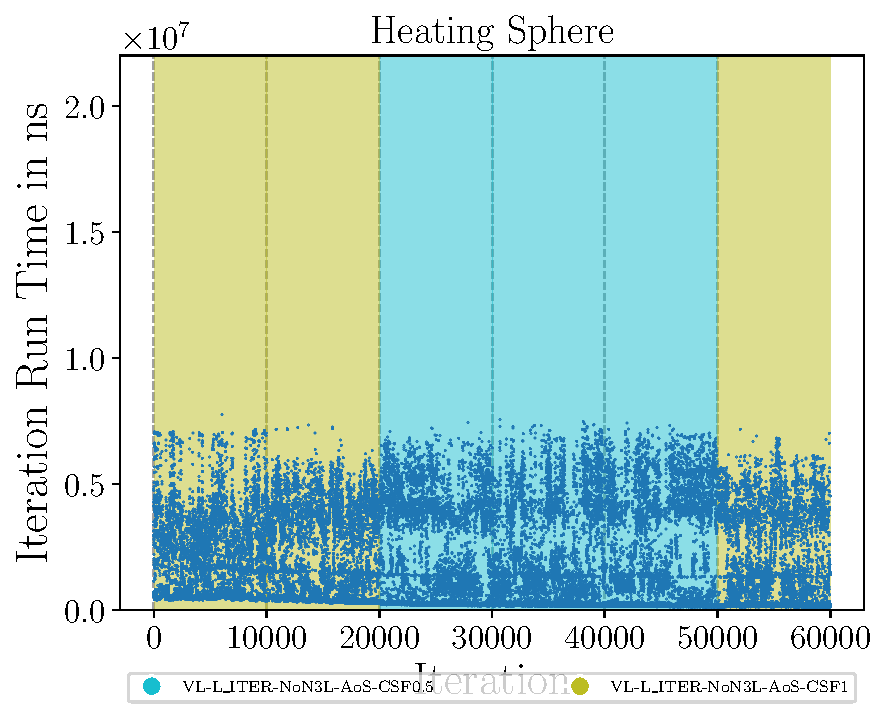
\includegraphics[width=\textwidth]{./plots/hs_vl_list_iter-non3l-aos_configs.pdf}
	\end{subfigure}%
	\begin{subfigure}{0.5\textwidth}
		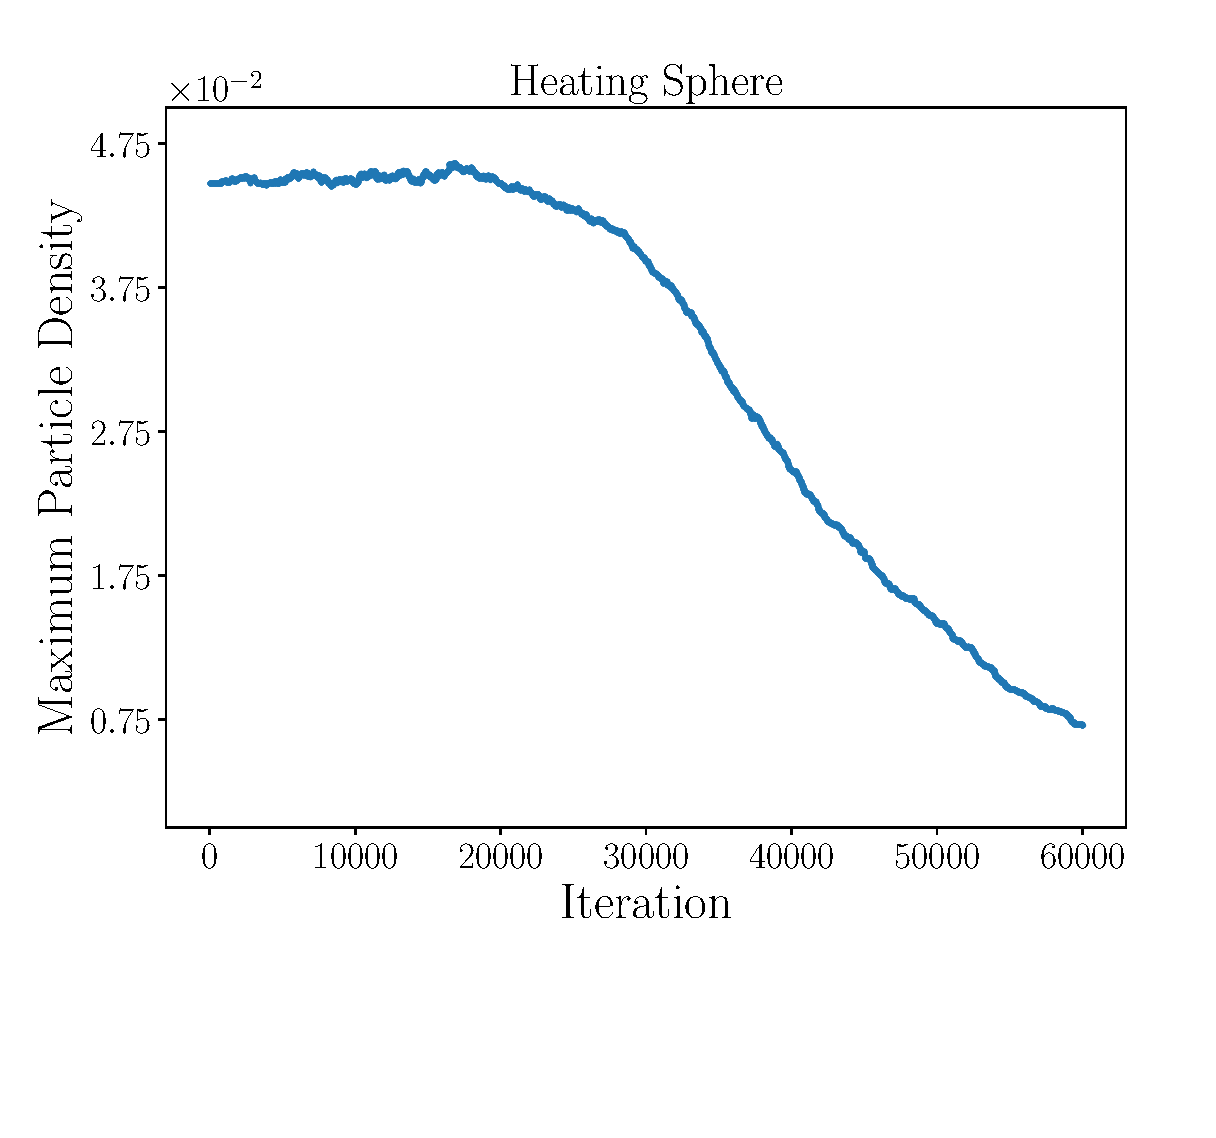
\includegraphics[width=\textwidth]{./plots/hs_vl_list_iter-non3l-aos_max_density.pdf}
	\end{subfigure}
	\begin{subfigure}{0.5\textwidth}
		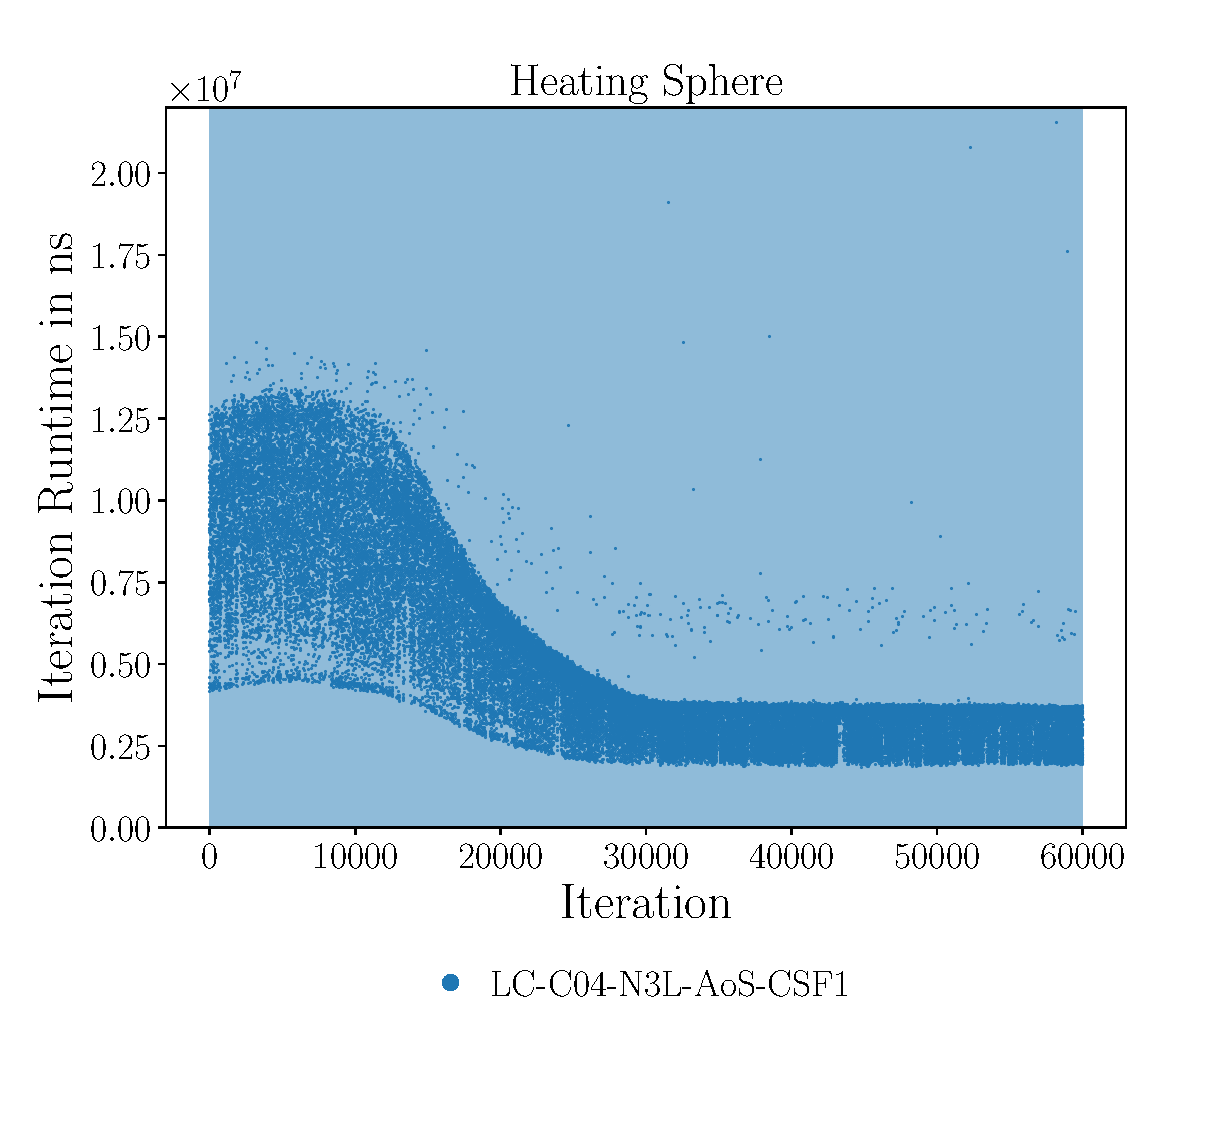
\includegraphics[width=\textwidth]{./plots/hs_lc_c04_n3l-aos-csf1_configs.pdf}
	\end{subfigure}%
	\begin{subfigure}{0.5\textwidth}
		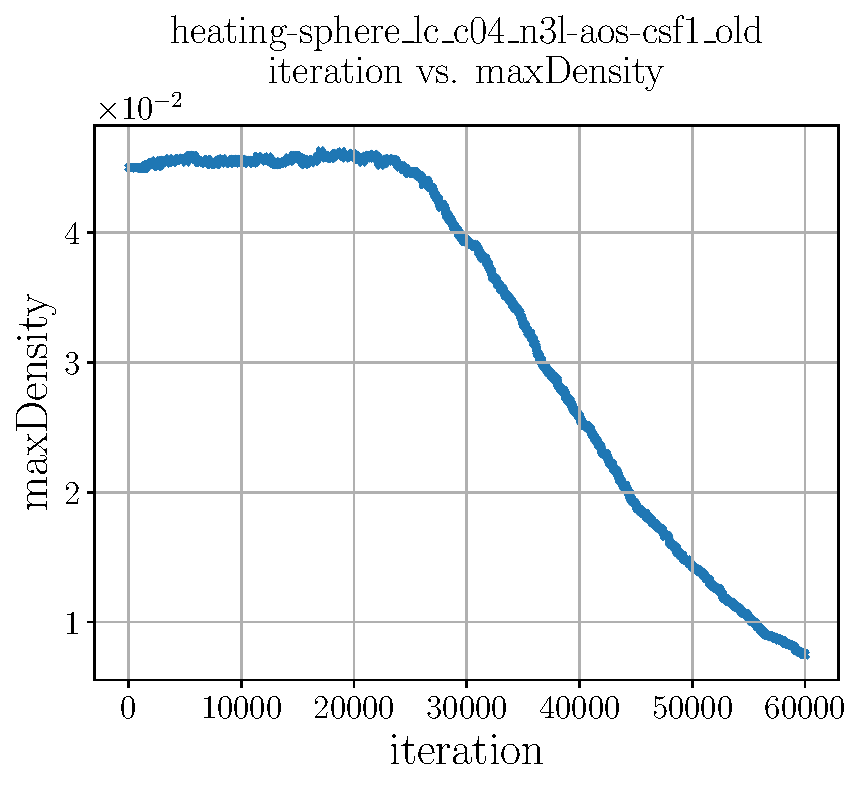
\includegraphics[width=\textwidth]{./plots/hs_lc_c04_n3l-aos-csf1_max_density.pdf}
	\end{subfigure}
	\caption{Iteration runtime (left) and the maximum densities of particles per cell (right). The top row shows a run with the single configuration \texttt{VL-List\_Iter-NoN3L-AoS}, the bottom row shows \texttt{LC-C04-N3L-AoS-CSF1}}
	\label{fig:liveinfo_heating_sphere}
\end{figure}





